\documentclass[aspectratio=169,10pt]{beamer}

% テーマとカラー設定
\usetheme{Madrid}
\usecolortheme{default}

% 日本語対応
\usepackage{luatexja}
\usepackage{luatexja-fontspec}

% 数式・図表パッケージ
\usepackage{amsmath}
\usepackage{graphicx}
\usepackage{booktabs}
\usepackage{multirow}

% 画像パス設定
\graphicspath{{./thesis-latex-template-251130/img/}}

% フッター設定
\setbeamertemplate{navigation symbols}{}
\setbeamertemplate{footline}[frame number]

% タイトル情報
\title{VRコンテンツ体験時における\\生体情報に基づく感情推定フレームワーク}
\author{趙 聖化 (27020856)}
\institute{関西学院大学 工学部 知能・機械工学課程\\指導教員: 井村 誠孝 教授}
\date{2026年3月1日}

\begin{document}

% タイトルスライド
\begin{frame}
\titlepage
\end{frame}

% 研究背景①
\begin{frame}{研究背景: VR技術の普及と課題}
\begin{block}{VR体験の広がり}
\begin{itemize}
\item HMDの普及により、ゲームや教育など様々な分野でVR体験が提供
\item ユーザに強い感情体験（恐怖、興奮、感動）を与えることが可能
\end{itemize}
\end{block}

\begin{alertblock}{従来の評価手法の限界}
\begin{itemize}
\item \textbf{アンケート・インタビュー}: 体験後の主観評価に依存
\begin{itemize}
\item バイアスや記憶の曖昧さが影響
\item リアルタイムの感情変化を捉えられない
\item 没入感を阻害する可能性
\end{itemize}
\end{itemize}
\end{alertblock}
\end{frame}

% 研究背景②
\begin{frame}{研究背景: 生体信号による客観的評価}
\begin{block}{生体信号の利点}
\begin{itemize}
\item \textbf{客観性}: 自律神経系の反応を直接測定
\item \textbf{非侵襲性}: VRの没入感を阻害しない
\item \textbf{リアルタイム性}: 瞬時の感情変化を捉えられる
\end{itemize}
\end{block}

\begin{columns}[T]
\column{0.33\textwidth}
\begin{block}{EDA}
皮膚電気活動\\
→ 覚醒度
\end{block}

\column{0.33\textwidth}
\begin{block}{ECG}
心電図\\
→ ストレス
\end{block}

\column{0.33\textwidth}
\begin{block}{EMG}
筋電図\\
→ 筋緊張
\end{block}
\end{columns}
\end{frame}

% 研究目的
\begin{frame}{研究目的}
\begin{block}{目標}
\Large
VR体験中のユーザの感情状態を\\
\textbf{リアルタイムに推定する}\\
マルチモーダルフレームワークの構築
\end{block}

\vspace{0.5cm}

\begin{itemize}
\item \textbf{生体信号} (EDA, ECG, EMG) の統合解析
\item \textbf{VRイベント}との同期
\item \textbf{機械学習}による自動感情推定
\item VRコンテンツの感情的効果の客観的評価
\end{itemize}
\end{frame}

% 関連研究①: 生体信号と行動指標
\begin{frame}{関連研究: 生体信号と行動指標による感情推定}
\begin{columns}[T]
\column{0.5\textwidth}
\begin{block}{生体信号 (Physiological)}
\begin{itemize}
\item \textbf{客観性}: 自律神経反応 (EDA, ECG, EMG) は偽装が困難 [Shu et al. 2018]
\item \textbf{VRとの親和性}: HMD装着時でも取得が容易 (顔表情認識の困難さを補完) [Hinkle et al. 2019]
\item \textbf{指標}: EDA(覚醒), ECG(ストレス), EMG(筋緊張)
\end{itemize}
\end{block}

\column{0.5\textwidth}
\begin{block}{行動指標 (Behavioral)}
\begin{itemize}
\item \textbf{トラッキング}: 頭部・手の動き、視線
\item \textbf{すくみ反応 (Freezing)}: 
\begin{itemize}
\item 強い恐怖に対する本能的な防御反応 [Pajić et al. 2025]
\item 身体硬直や操作停止として現れる [Lin 2017]
\end{itemize}
\end{itemize}
\end{block}
\end{columns}

\vspace{0.1cm}
\hrule
\vspace{0.1cm}
\tiny
\noindent [Shu et al. 2018] L. Shu et al. A Review of Emotion Recognition Using Physiological Signals, Sensors, 18(7):2074 (2018)\\
\noindent [Hinkle et al. 2019] L. B. Hinkle et al. Physiological Measurement for Emotion Recognition in Virtual Reality, ICDIS, pp. 136–143 (2019)\\
\noindent [Pajić et al. 2025] D. Pajić et al. Risky behavior in virtual reality: The roles of personality, environment, and physiology, PLoS ONE, 20(1):e0316896 (2025)\\
\noindent [Lin 2017] J. H. T. Lin. Fear in Virtual Reality (VR): Fear elements... Computers in Human Behavior, 72:350–361 (2017)
\end{frame}

% 関連研究②: マルチモーダル統合と本研究の位置づけ
\begin{frame}{関連研究: マルチモーダル統合と本研究の位置づけ}
\begin{block}{マルチモーダル推定の利点}
\begin{itemize}
\item 単一指標よりも推定精度が向上 (例: ECG+GSRで高精度化 [Dar et al. 2020])
\item 生体情報とシステムが相互作用する「アフェクティブ・ループ」の基盤 [Marín-Morales et al. 2020]
\end{itemize}
\end{block}

\begin{alertblock}{既存研究の課題 $\rightarrow$ 本研究のアプローチ}
\begin{itemize}
\item \textbf{課題}: 多くの研究はオフライン解析が主で、\textbf{イベントとの厳密なリアルタイム同期}が不足
\item \textbf{本研究}: 
\begin{itemize}
\item 生体信号(1kHz)とVRイベントをTCP通信で\textbf{ミリ秒単位同期}
\item 恐怖・驚き・集中を対象とした統合フレームワークの構築
\end{itemize}
\end{itemize}
\end{alertblock}

\vspace{0.2cm}
\hrule
\vspace{0.1cm}
\tiny
\noindent [Dar et al. 2020] M. N. Dar et al. CNN and LSTM-Based Emotion Charting Using Physiological Signals, Sensors, 20(16):4551 (2020)\\
\noindent [Marín-Morales et al. 2020] J. Marín-Morales et al. Emotion Recognition in Immersive Virtual Reality: From Statistics to Affective Computing, Sensors, 20(18):5163 (2020)
\end{frame}

% 提案手法①: システムアーキテクチャ
\begin{frame}{提案手法: システムアーキテクチャ}
\begin{columns}[T]
\column{0.5\textwidth}
\begin{block}{Unity (VRクライアント)}
\begin{itemize}
\item Meta Quest Pro
\item イベント発生検出
\item TCPでマーカー送信
\end{itemize}
\end{block}

\begin{block}{Python (解析サーバ)}
\begin{itemize}
\item BITalinoデータ収集
\item イベント同期
\item 特徴量抽出
\end{itemize}
\end{block}

\column{0.5\textwidth}
\begin{figure}
\centering
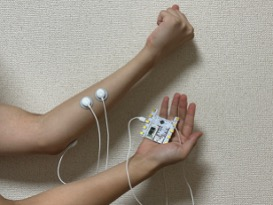
\includegraphics[width=0.3\textwidth]{EMG.jpg}
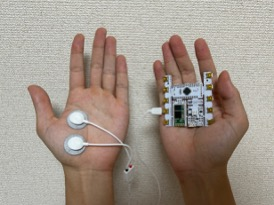
\includegraphics[width=0.3\textwidth]{EDA.jpg}
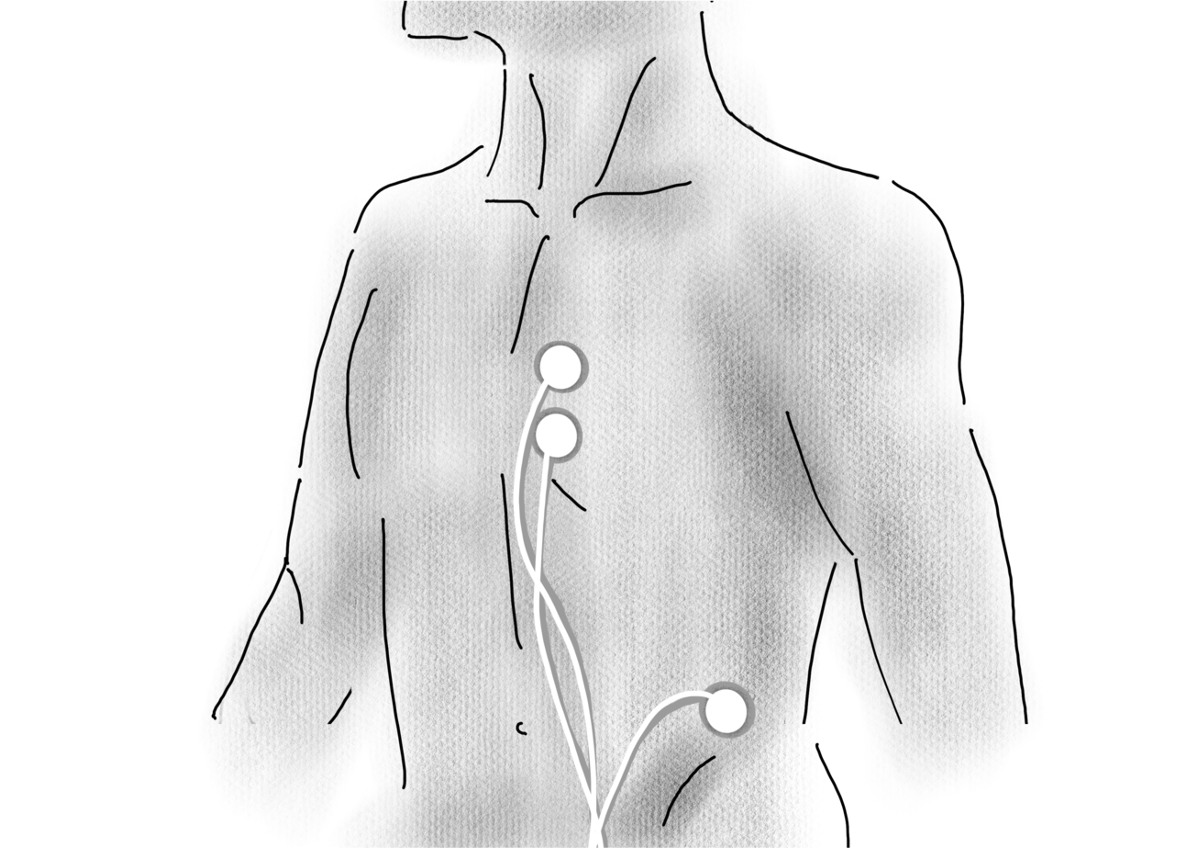
\includegraphics[width=0.3\textwidth]{ECG.png}
\caption*{センサ装着位置: EMG, EDA, ECG}
\end{figure}
\end{columns}

\vspace{0.3cm}
\begin{center}
\textbf{TCP/IP通信により1kHzでリアルタイム同期}
\end{center}
\end{frame}

% 提案手法②: 測定指標
\begin{frame}{提案手法: 測定指標と特徴量}
\begin{table}
\scriptsize
\begin{tabular}{lll}
\toprule
\textbf{信号} & \textbf{特徴量} & \textbf{生理学的意義} \\
\midrule
\multirow{3}{*}{ECG} & 心拍数 (HR) & 全般的覚醒水準 \\
& RMSSD & 副交感神経活動 \\
& LF/HF比 & 自律神経バランス \\
\midrule
\multirow{2}{*}{EMG} & RMS電圧 & 筋活動エネルギー \\
& 最大電圧 & 筋活動ピーク強度 \\
\midrule
\multirow{2}{*}{EDA} & 平均SCL & 基礎的覚醒水準 \\
& SCRパルス数 & 刺激反応頻度 \\
\bottomrule
\end{tabular}
\end{table}

\vspace{0.3cm}
\begin{center}
\textbf{合計20個の生理学的特徴量を抽出}
\end{center}
\end{frame}

% 実験設計
\begin{frame}{実験設計: 4段階VRホラーシナリオ}
\begin{table}
\scriptsize
\begin{tabular}{clll}
\toprule
\textbf{Phase} & \textbf{環境・課題} & \textbf{誘導感情} & \textbf{予想される反応} \\
\midrule
Phase 0 & 暗い部屋、十字注視 (60秒) & 安定 (Rest) & ベースライン測定 \\
Phase 1 & Go/No-Go課題 & 集中 (Focus) & 認知負荷 \\
Phase 2 & 暗い屋敷、アイテム収集 & 不安/恐怖 & SCL漸進的上昇 \\
Phase 3 & ゾンビ追跡、脱出 & 恐怖/驚き & HR, SCL, EMG急増 \\
\bottomrule
\end{tabular}
\end{table}

\vspace{0.3cm}
\begin{columns}[T]
\column{0.25\textwidth}
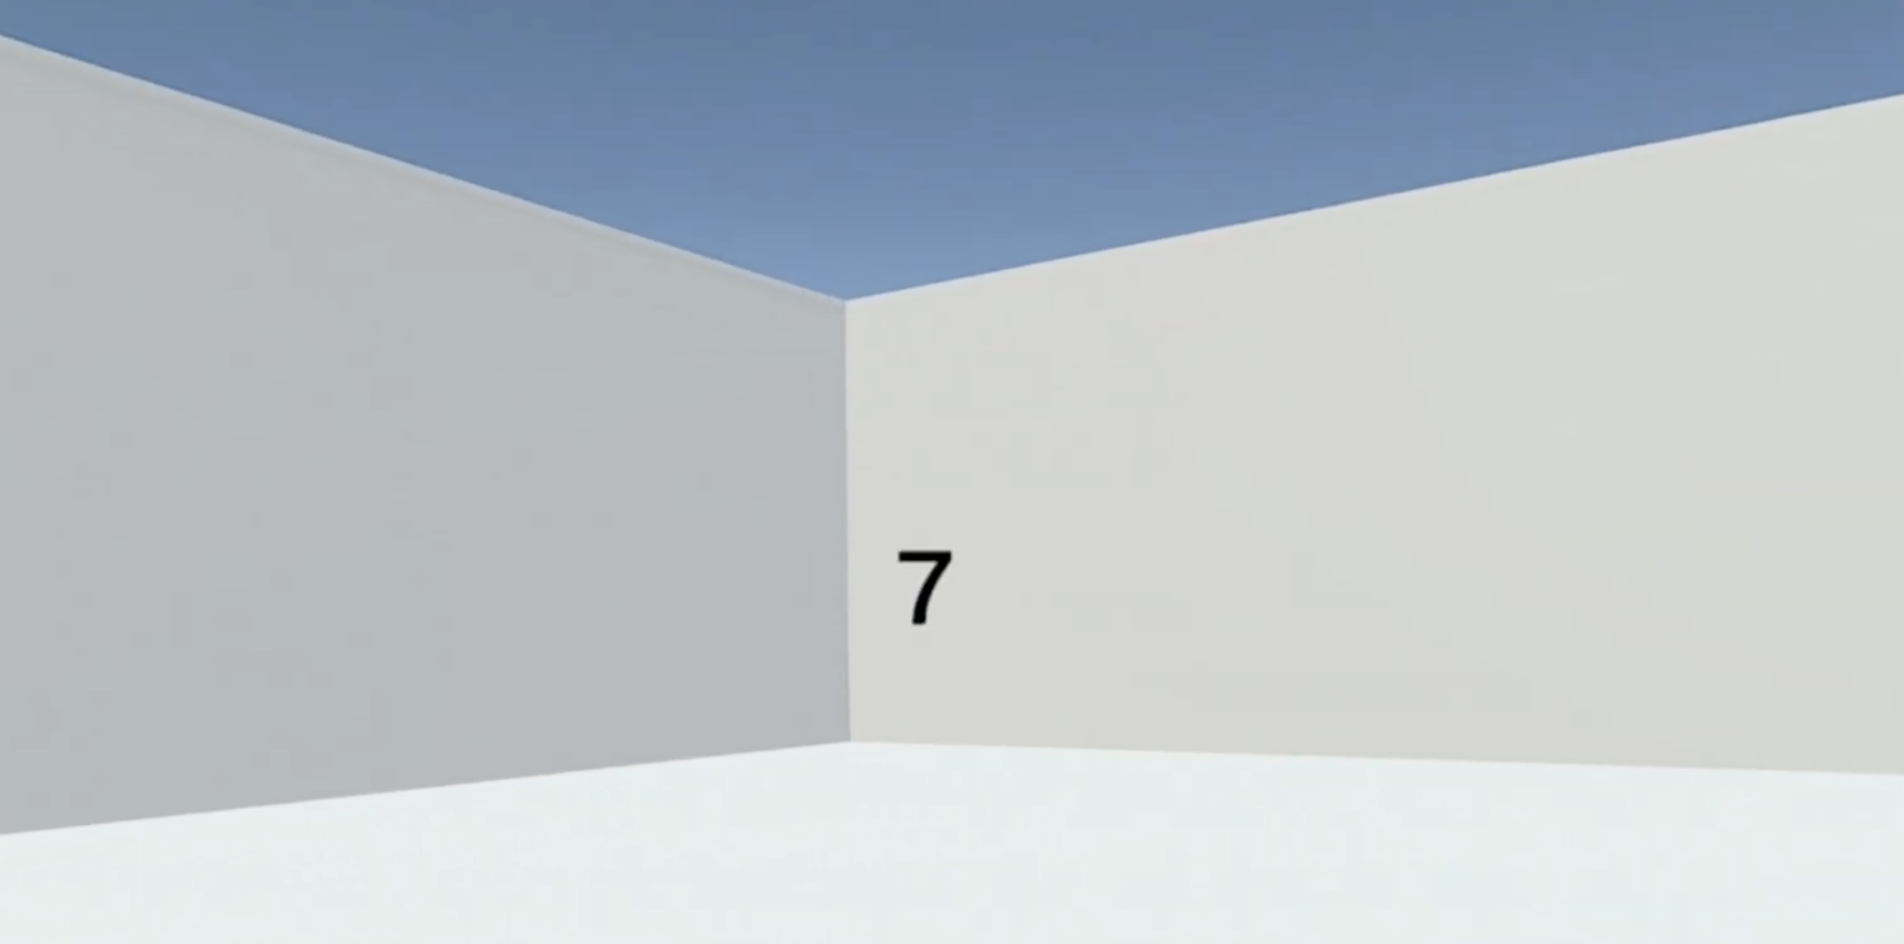
\includegraphics[width=\textwidth]{phase0_baseline.png}
\tiny Phase 0

\column{0.25\textwidth}
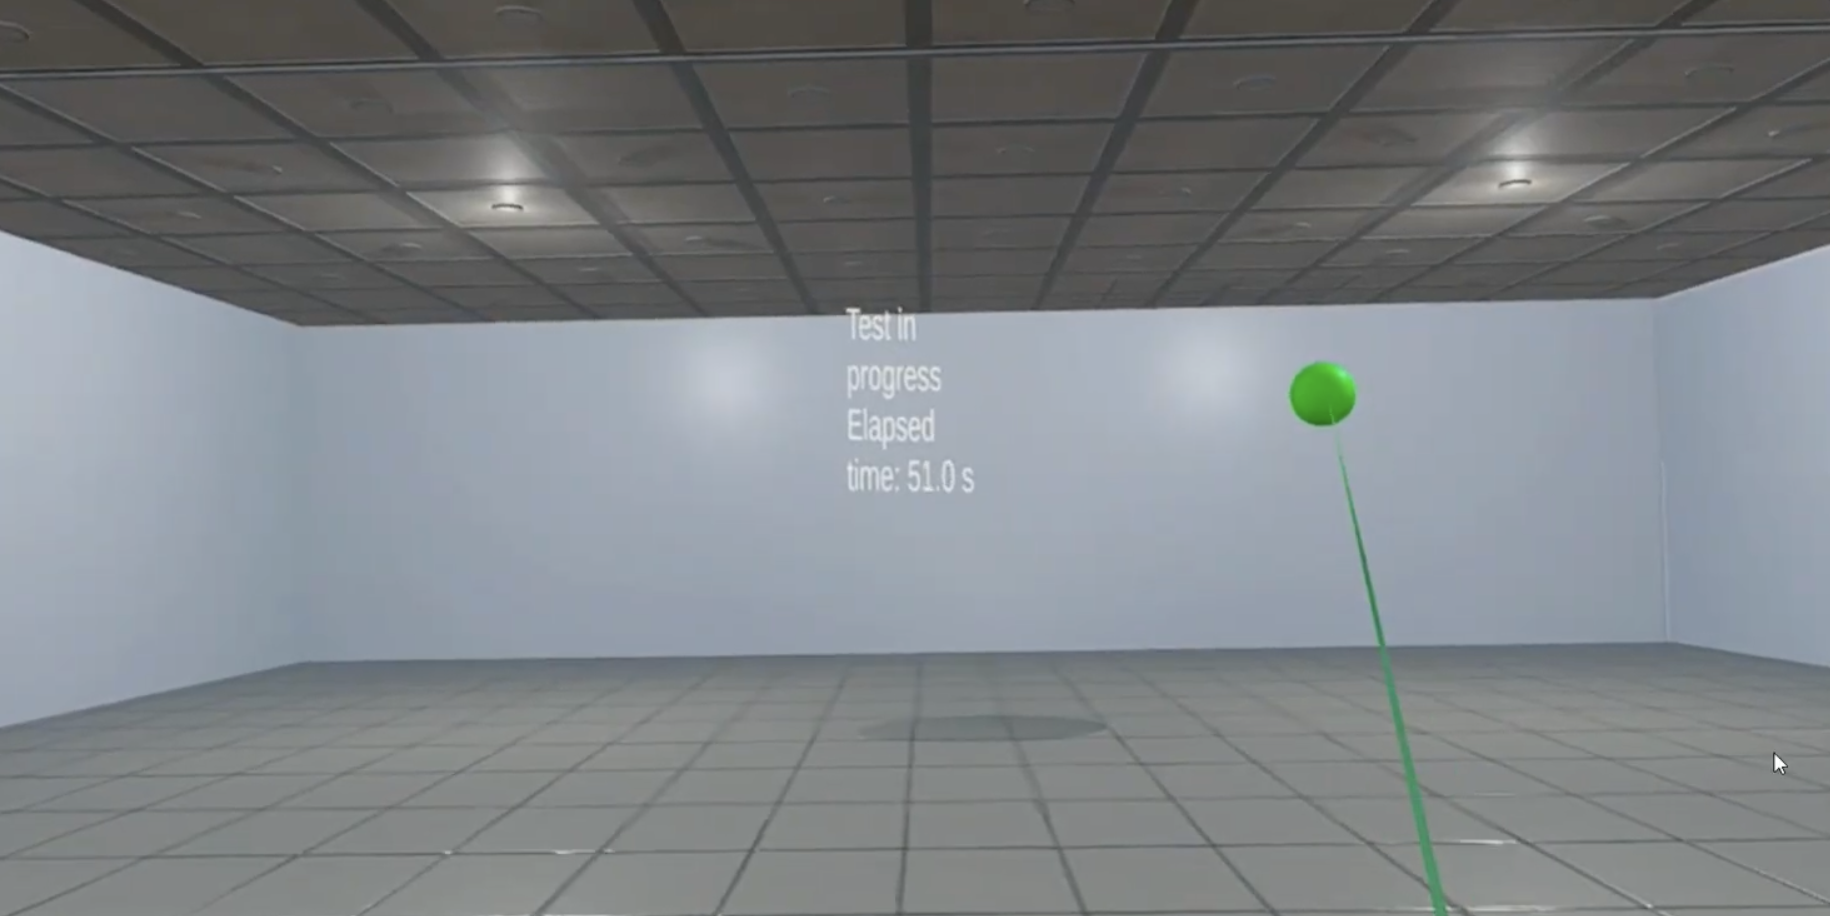
\includegraphics[width=\textwidth]{phase1_go.png}
\tiny Phase 1

\column{0.25\textwidth}
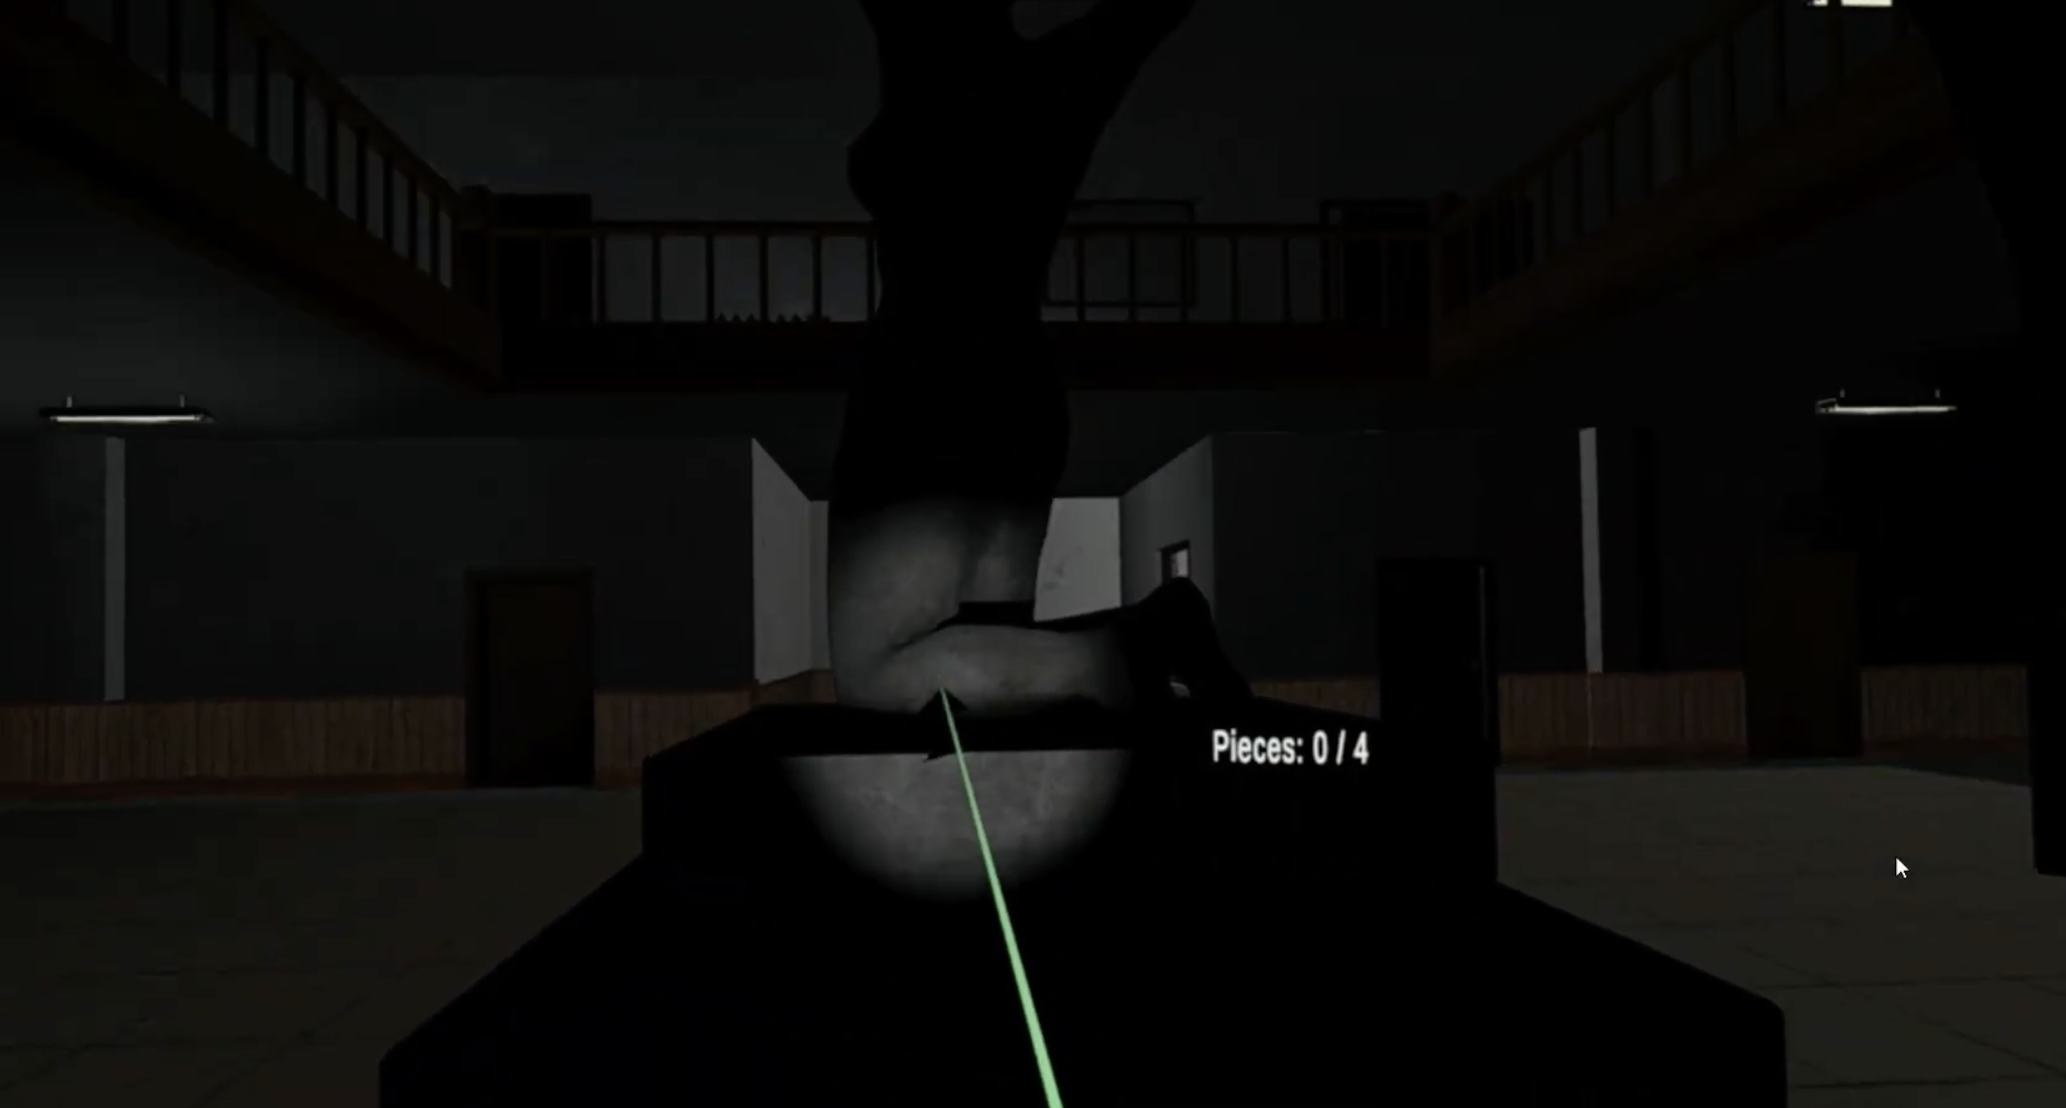
\includegraphics[width=\textwidth]{phase2_map.png}
\tiny Phase 2

\column{0.25\textwidth}
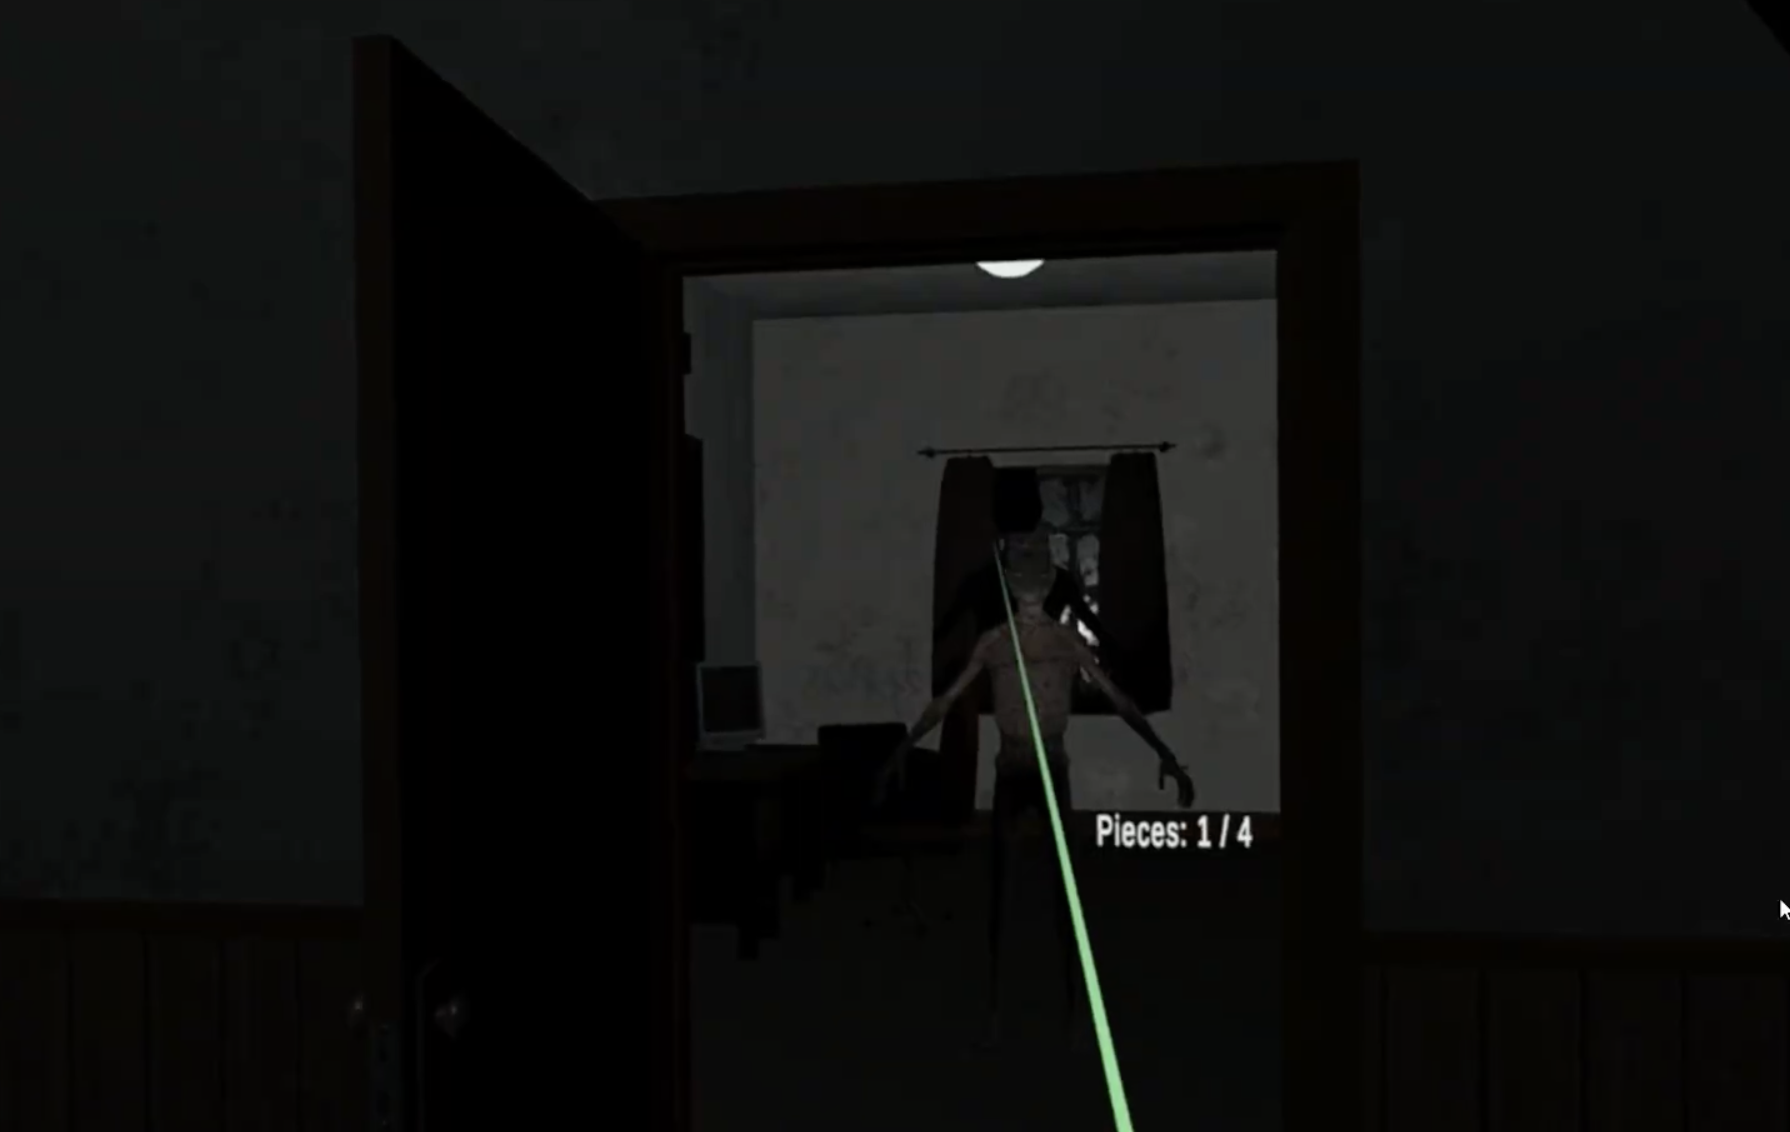
\includegraphics[width=\textwidth]{phase2_zombie.png}
\tiny Phase 3
\end{columns}

\vspace{0.2cm}
\begin{center}
\textbf{参加者: 6名、8セッション}
\end{center}
\end{frame}

% 実験結果①: 生体反応の変化
\begin{frame}{実験結果①: 生体反応の変化}
\begin{figure}
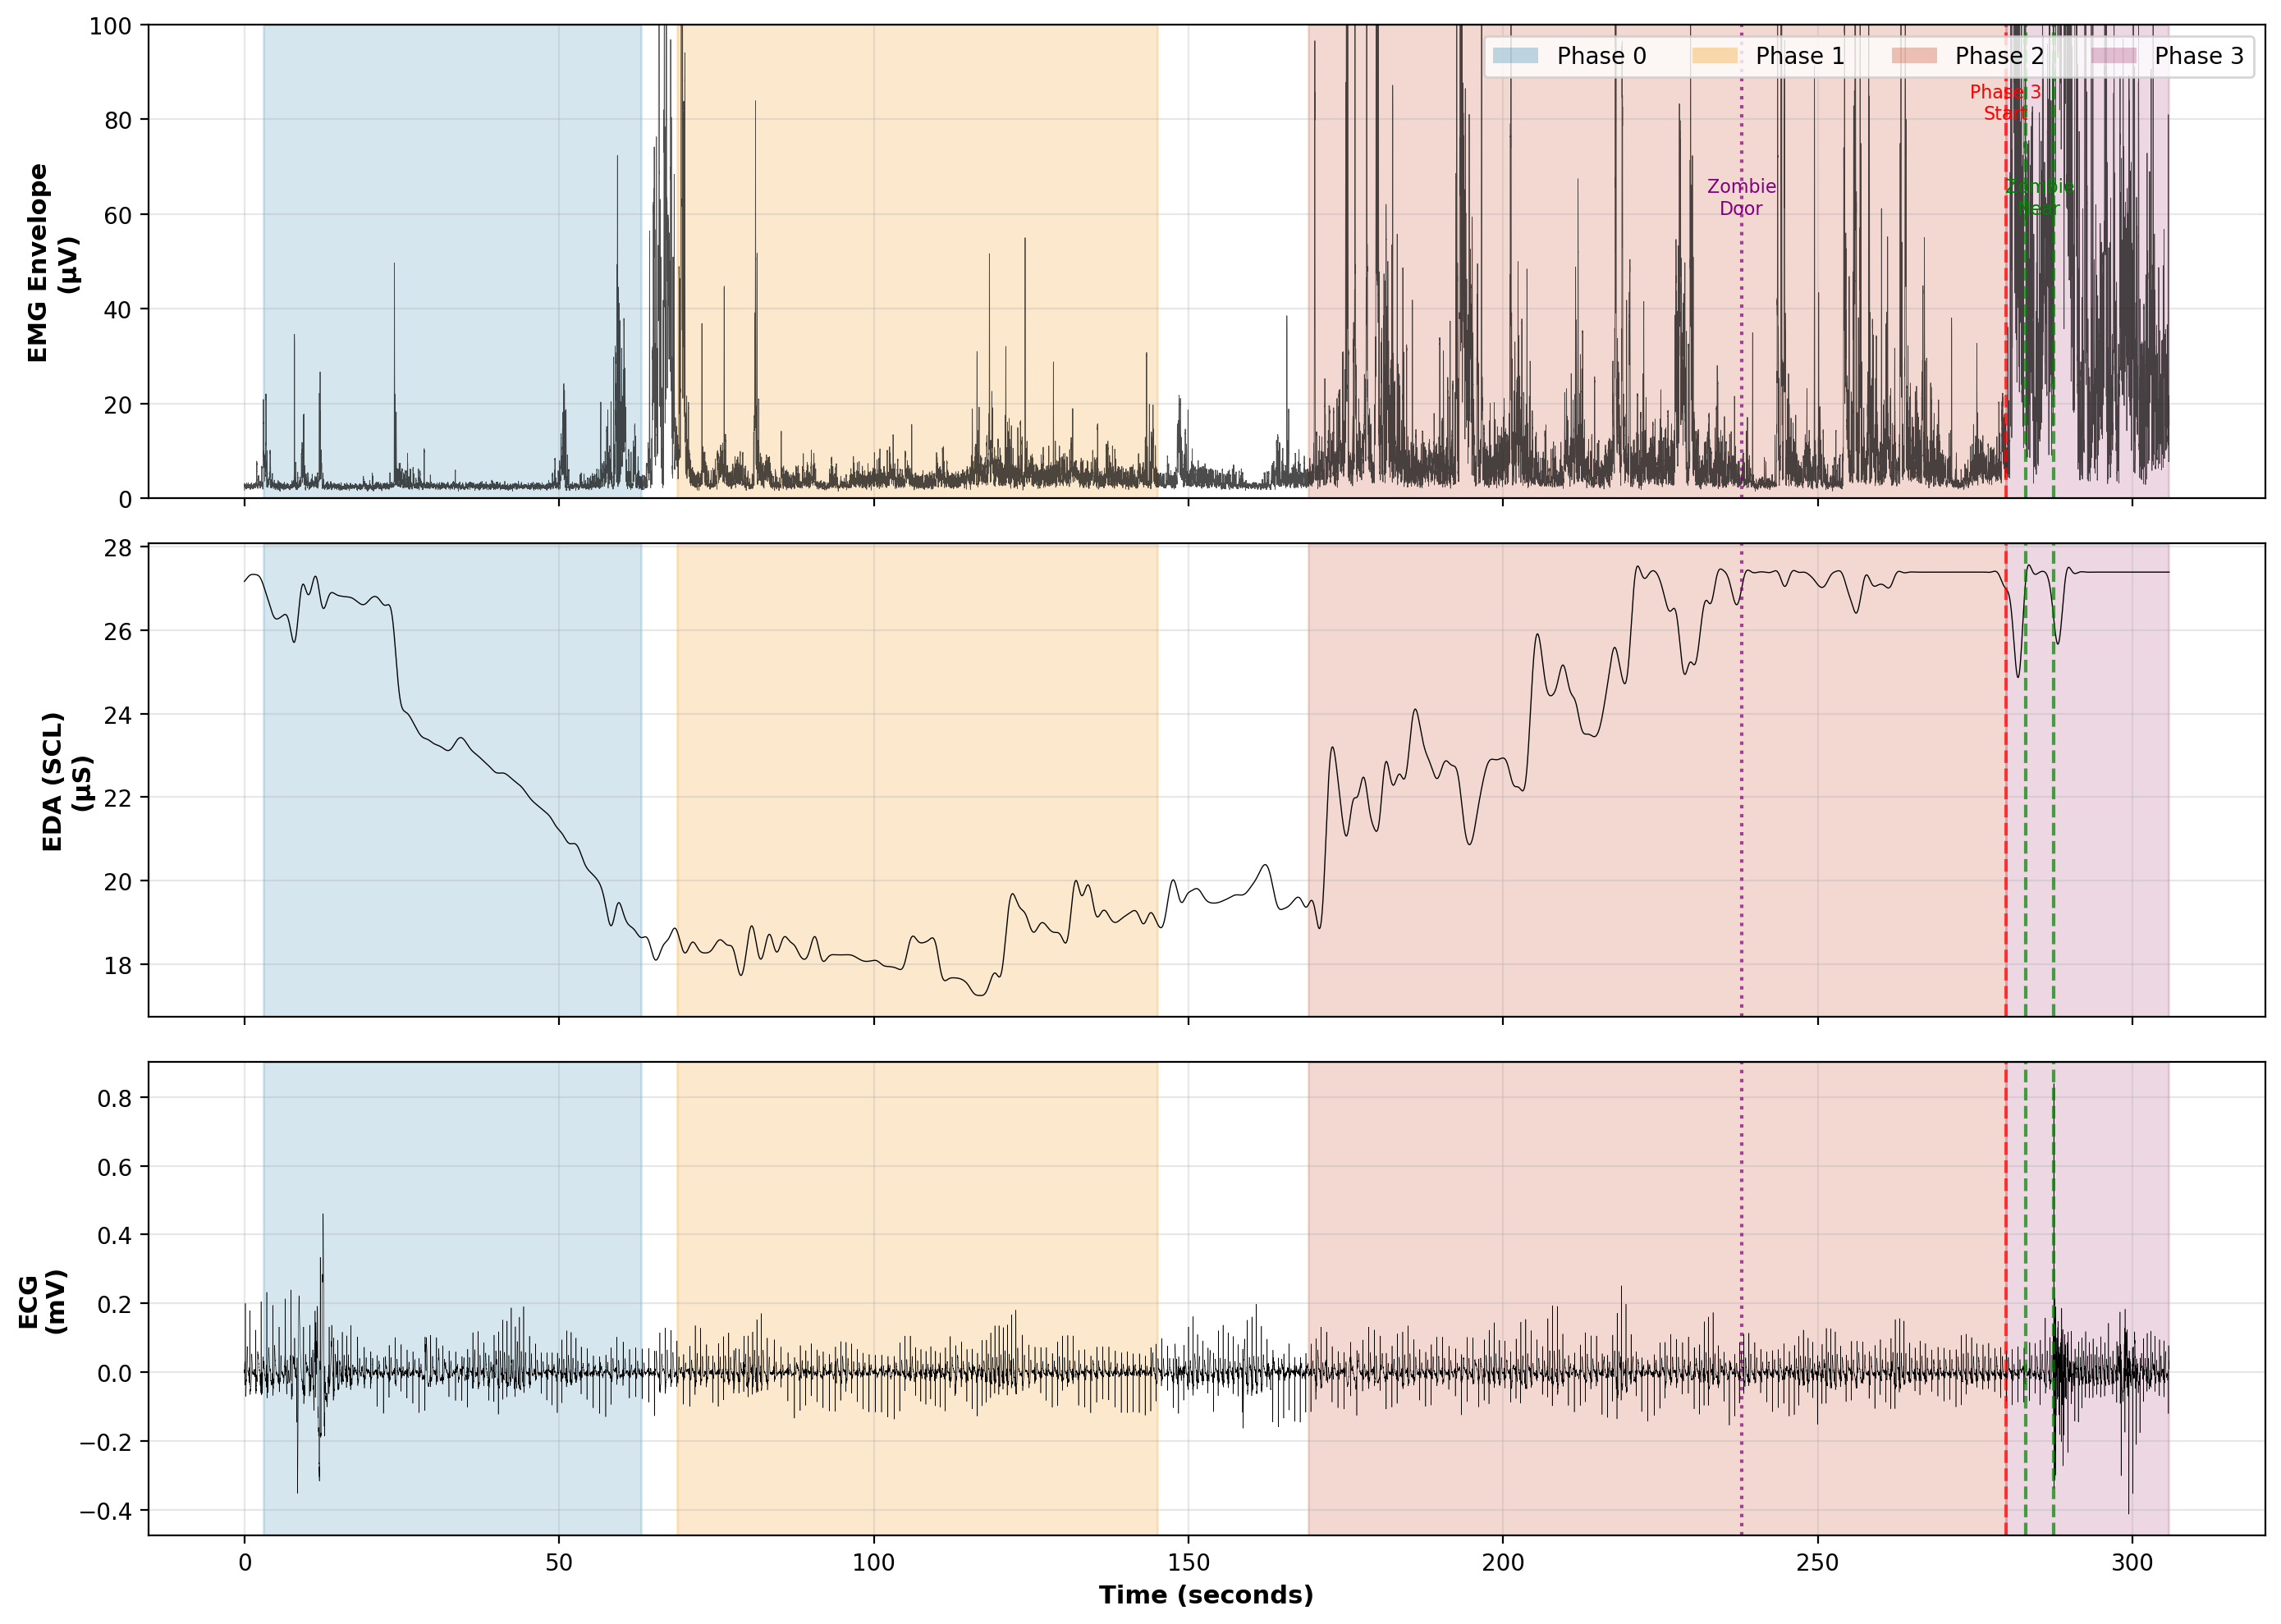
\includegraphics[width=0.95\textwidth]{fig1_continuous_data.png}
\caption*{連続生体信号記録 (Subject E2)}
\end{figure}

\begin{itemize}
\item \textbf{SCL}: Phase 2-3で顕著な上昇 (22.2 → 26.6 $\mu$S)
\item \textbf{EMG}: Phase 3で\textcolor{red}{2倍以上}に増加 (16.9 → 36.0 $\mu$V)
\item \textbf{HR}: 個人差が大きい（すくみ反応の観察）
\end{itemize}
\end{frame}

% 実験結果②: Phase別統計
\begin{frame}{実験結果②: Phase別統計}
\begin{columns}[T]
\column{0.5\textwidth}
\begin{table}
\tiny
\caption*{Phase別生体反応 (Mean $\pm$ SD)}
\begin{tabular}{lcccc}
\toprule
特徴量 & P0 & P1 & P2 & P3 \\
\midrule
HR (bpm) & 73.0 & 74.2 & 76.5 & 72.2 \\
RMSSD (ms) & 143.3 & 51.4 & 67.0 & \textcolor{red}{742.4} \\
SCL ($\mu$S) & 22.2 & 20.9 & \textcolor{blue}{26.6} & \textcolor{blue}{26.7} \\
EMG RMS & 16.9 & 18.2 & 25.4 & \textcolor{red}{36.0} \\
\bottomrule
\end{tabular}
\end{table}

\column{0.5\textwidth}
\begin{figure}
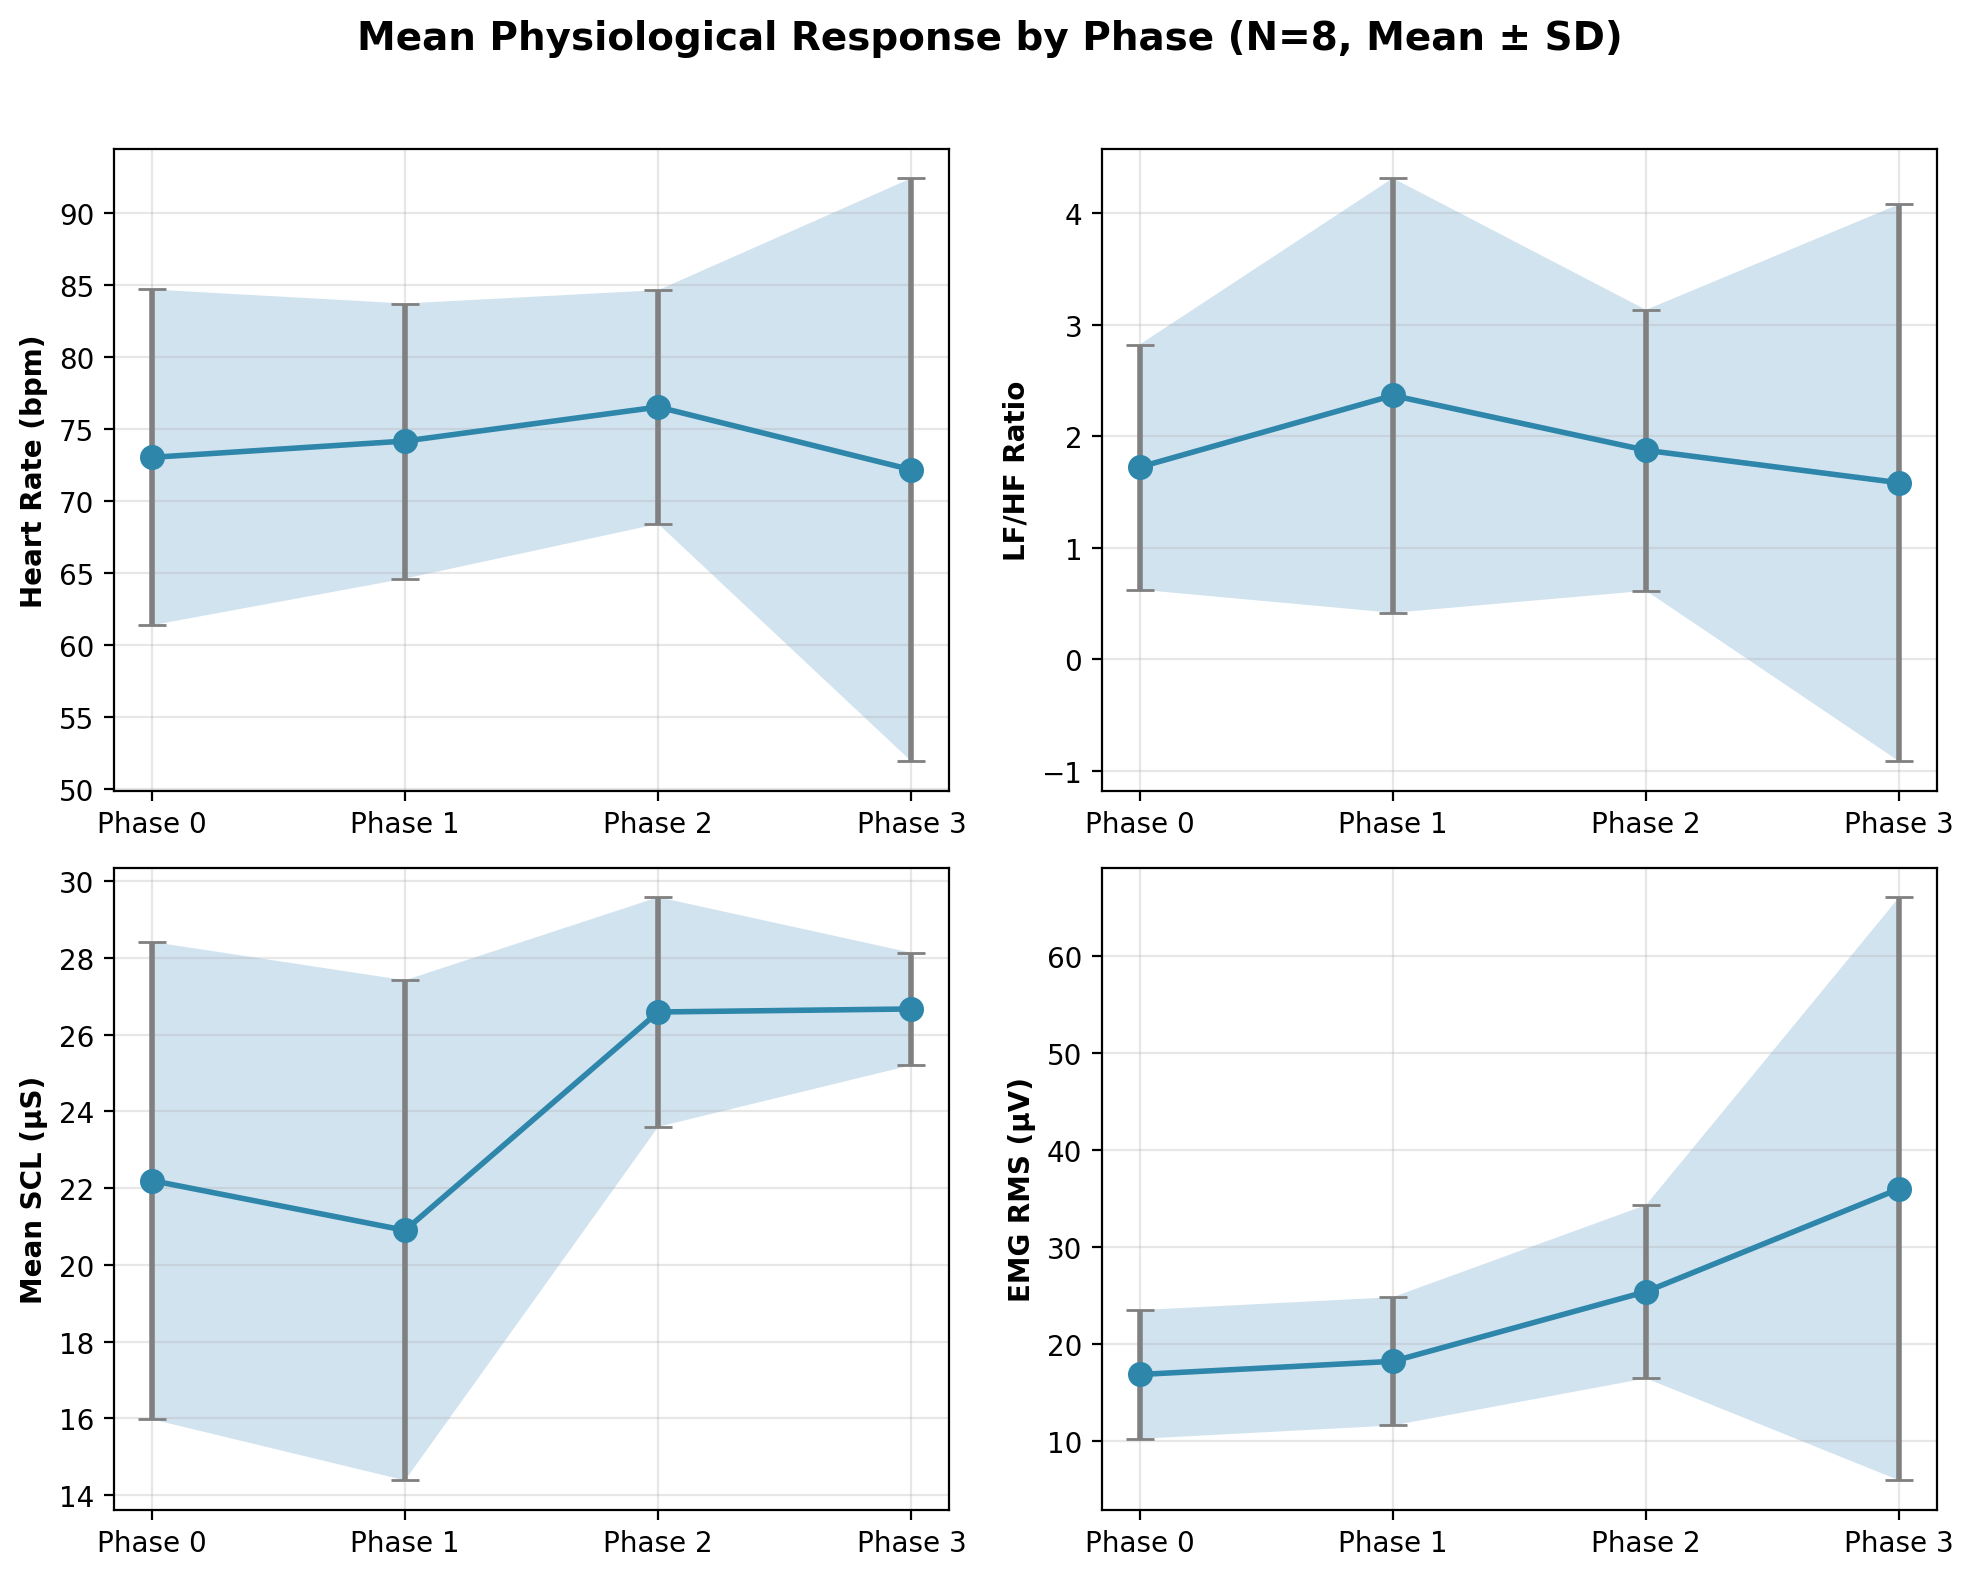
\includegraphics[width=\textwidth]{fig6_phase_mean.png}
\end{figure}
\end{columns}

\vspace{0.3cm}
\begin{alertblock}{主要な発見}
\begin{itemize}
\item SCL・EMGは恐怖に対して\textbf{一貫した上昇}
\item HRVは\textbf{個人差が大きい}（すくみ反応の影響）
\end{itemize}
\end{alertblock}
\end{frame}

% 実験結果③: 機械学習分類
\begin{frame}{実験結果③: 機械学習によるPhase分類}
\begin{columns}[T]
\column{0.5\textwidth}
\begin{block}{Random Forestモデル}
\begin{itemize}
\item \textbf{Accuracy: 67.7\%}
\item ランダム確率(25\%)の\textcolor{red}{2.7倍}
\item Leave-One-Session-Out検証
\end{itemize}
\end{block}

\begin{table}
\tiny
\begin{tabular}{lcc}
\toprule
Phase & Recall & 識別性能 \\
\midrule
Phase 0 & \textcolor{blue}{88\%} & 優秀 \\
Phase 1 & 38\% & 低い \\
Phase 2 & 75\% & 良好 \\
Phase 3 & \textcolor{blue}{71\%} & 良好 \\
\bottomrule
\end{tabular}
\end{table}

\column{0.5\textwidth}
\begin{figure}
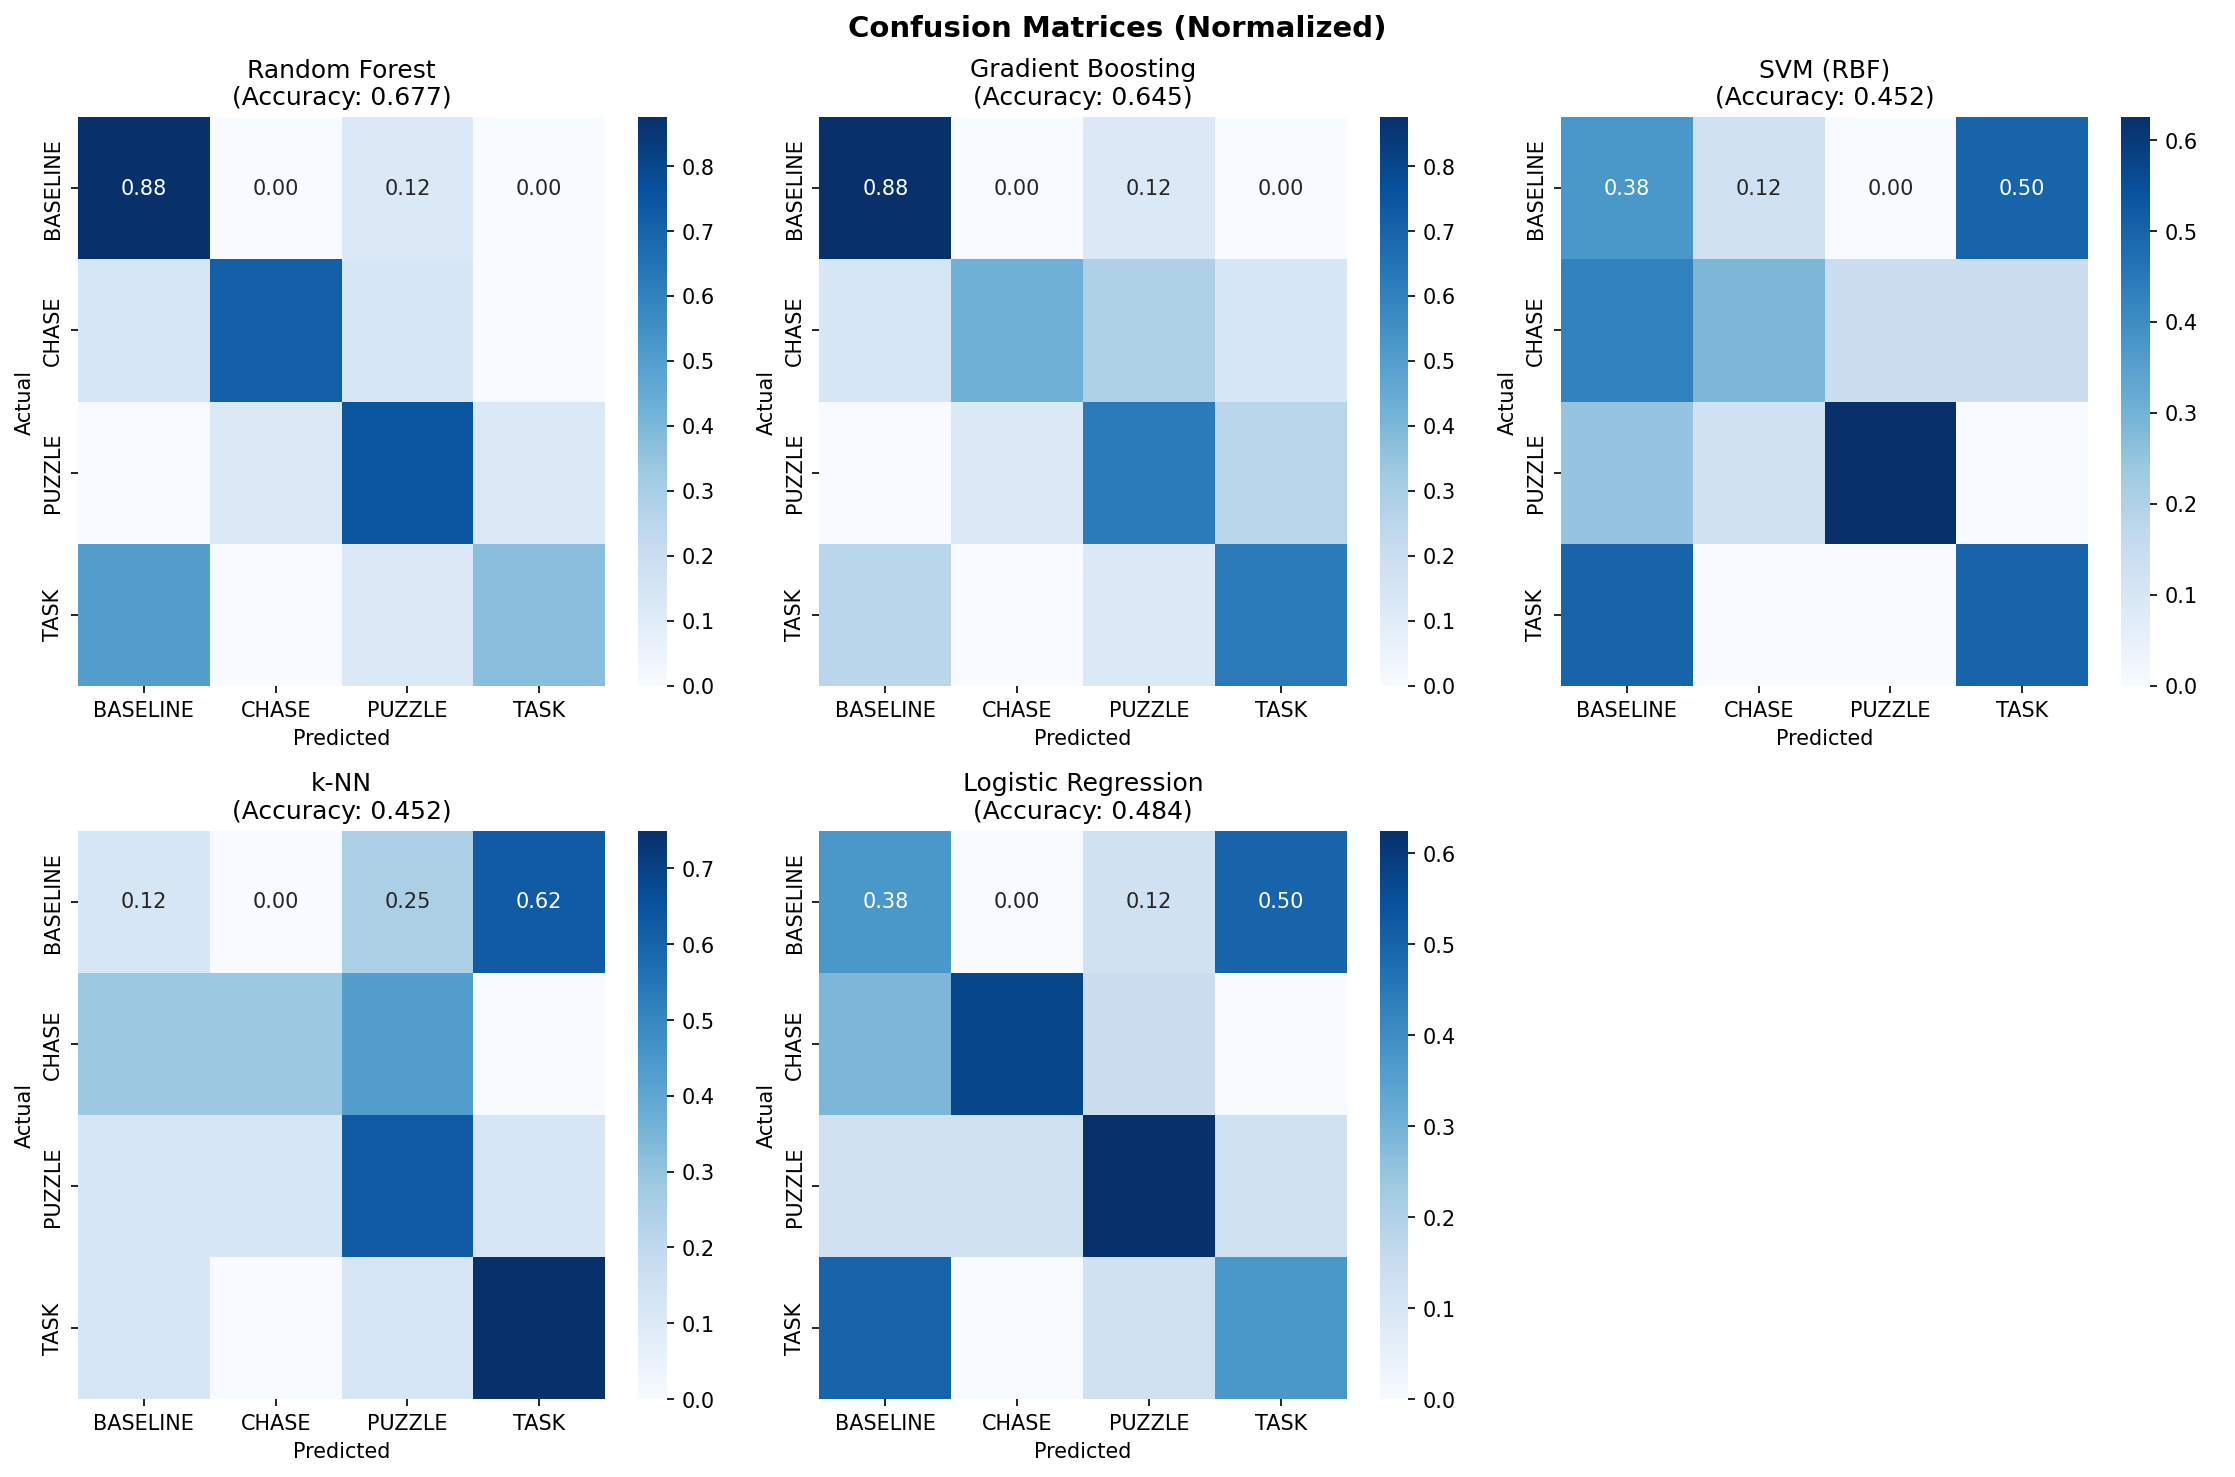
\includegraphics[width=\textwidth]{fig8_confusion_matrices.png}
\caption*{混同行列}
\end{figure}
\end{columns}
\end{frame}

% 実験結果④: 特徴量重要度
\begin{frame}{実験結果④: 特徴量重要度分析}
\begin{figure}
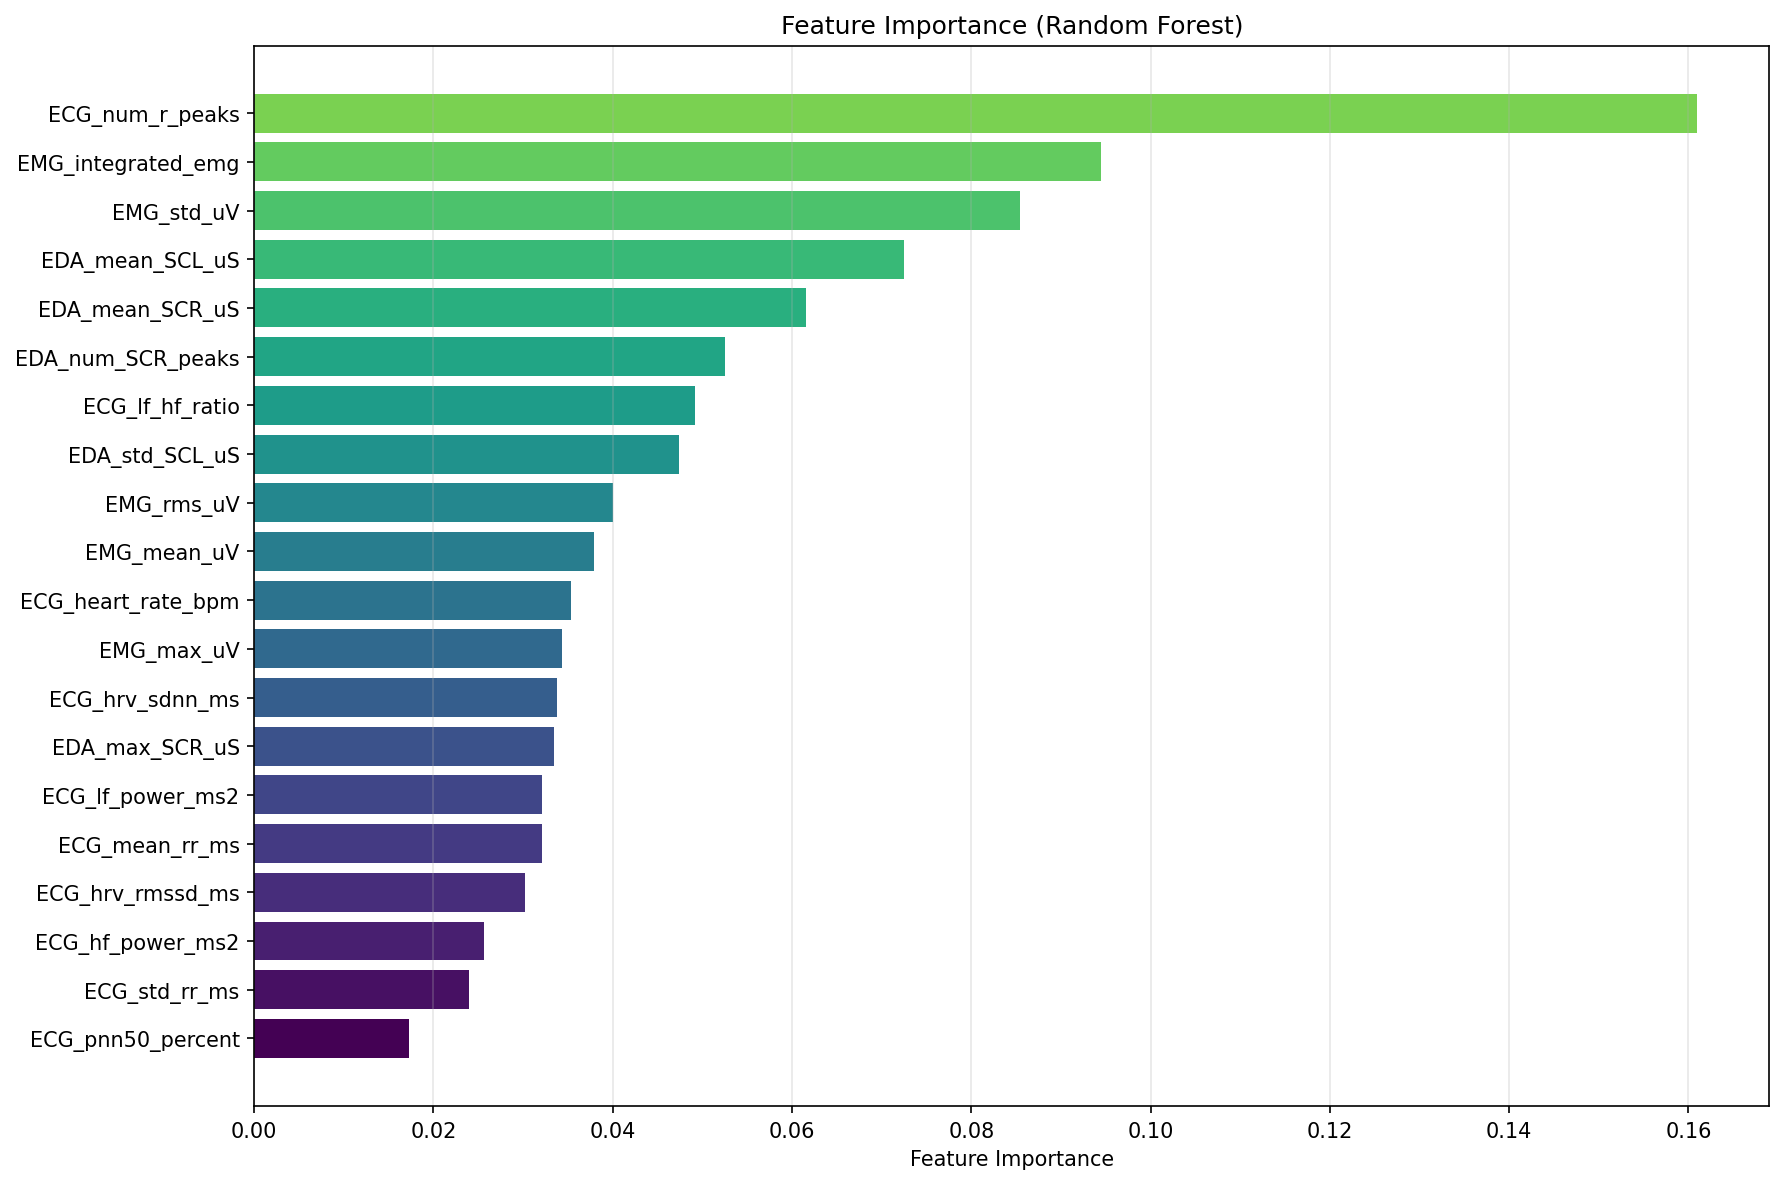
\includegraphics[width=0.8\textwidth]{fig9_feature_importance.png}
\end{figure}

\begin{block}{重要な特徴量 (上位5つ)}
\begin{enumerate}
\item \textbf{EMG積分値} (9.3\%): 累積筋活動量
\item \textbf{EMG標準偏差} (8.0\%): 筋活動の変動性
\item \textbf{EDA平均SCL} (7.2\%): 平均皮膚電気伝導度
\item \textbf{EDA平均SCR} (5.8\%): 平均皮膚電気反応
\end{enumerate}
\end{block}

\begin{center}
\textbf{→ EMGとEDAが感情状態識別に有効}
\end{center}
\end{frame}

% 考察
\begin{frame}{考察: すくみ (Freezing) 反応の観察}
\begin{columns}[T]
\column{0.5\textwidth}
\begin{block}{Subject E2の事例}
\begin{itemize}
\item 主観評価: 恐怖度\textcolor{red}{7点/7点}
\item 心拍数: 28.96 bpmまで\textbf{低下}
\item EMG RMS: 57.01 $\mu$V (\textbf{平均の1.5倍})
\end{itemize}
\end{block}

\begin{alertblock}{解釈}
「\textbf{恐怖誘発性徐脈}」\\
= すくみ反応
\begin{itemize}
\item 副交感神経が強く活性化
\item 外見上は静止
\item 体内では著しく緊張
\end{itemize}
\end{alertblock}

\column{0.5\textwidth}
\begin{block}{個人差の類型}
\begin{enumerate}
\item \textbf{没入型恐怖反応群}\\
(A, B, C, E)\\
→ 生体反応が顕著

\item \textbf{認知失敗群} (D, F)\\
→ 追跡を認知できず

\item \textbf{無意識的緊張維持} (F)\\
→ 意識的には気づかないが\\
\quad 身体は緊張状態
\end{enumerate}
\end{block}
\end{columns}

\vspace{0.3cm}
\begin{center}
\textbf{→ マルチモーダル統合により、意識・無意識の両方を捕捉可能}
\end{center}
\end{frame}

% 結論
\begin{frame}{結論}
\begin{block}{達成できたこと}
\begin{itemize}
\item \textbf{マルチモーダル感情推定フレームワーク}の構築
\begin{itemize}
\item 生体信号 (EDA, ECG, EMG) とVRイベントのリアルタイム同期
\item TCP/IP通信による1kHz高精度データ収集
\end{itemize}
\item \textbf{機械学習による自動Phase分類}
\begin{itemize}
\item Random Forest: Accuracy 67.7\% (ランダムの2.7倍)
\item 安定状態・恐怖状態の高精度識別 (Recall 88\%, 71\%)
\end{itemize}
\item \textbf{すくみ反応など深層的感情反応}の客観的検出
\end{itemize}
\end{block}

\begin{alertblock}{今後の課題}
\begin{itemize}
\item データ規模の拡大（より多くの参加者）
\item 動きノイズ除去の強化（加速度センサ活用）
\item リアルタイム推定システムへの発展（スライディングウィンドウ）
\item 個人適応型キャリブレーション機能の実装
\end{itemize}
\end{alertblock}
\end{frame}

% 社会的意義
\begin{frame}{社会的意義と応用分野}
\begin{columns}[T]
\column{0.33\textwidth}
\begin{block}{医療・心理治療}
\begin{itemize}
\item PTSD治療
\item 不安障害治療
\item VR暴露療法
\end{itemize}
\vspace{0.2cm}
→ ストレスレベルを\\
\quad リアルタイム\\
\quad モニタリング
\end{block}

\column{0.33\textwidth}
\begin{block}{教育・訓練}
\begin{itemize}
\item 手術シミュレーション
\item 危険予知訓練
\item 特殊教育
\end{itemize}
\vspace{0.2cm}
→ 認知負荷を\\
\quad 客観的評価、\\
\quad 個別フィードバック
\end{block}

\column{0.33\textwidth}
\begin{block}{次世代UX}
\begin{itemize}
\item コンテンツ制作
\item メタバース
\item ソーシャルVR
\end{itemize}
\vspace{0.2cm}
→ アフェクティブ\\
\quad ・ループの実現、\\
\quad 適応型コンテンツ
\end{block}
\end{columns}

\vspace{0.5cm}
\begin{center}
\Large
\textbf{VR体験の質的向上と新たな可能性の創出}
\end{center}
\end{frame}

% 謝辞
\begin{frame}{謝辞}
\begin{center}
\Large
本研究を進めるにあたり、\\
終始懇切丁寧なるご指導とご鞭撻を賜りました\\
\vspace{0.5cm}

\textbf{関西学院大学 工学部}\\
\textbf{知能・機械工学課程}\\
\vspace{0.3cm}

\textbf{井村 誠孝 教授}\\
\vspace{0.3cm}

に、謹んで深甚なる謝意を表します。\\
\vspace{0.5cm}

また、実験にご協力いただきました\\
参加者の皆様に深く感謝申し上げます。
\end{center}
\end{frame}

% 参考文献
\begin{frame}[allowframebreaks]{参考文献}
\bibliographystyle{plain}
\bibliography{reference}
\end{frame}

\end{document}
